\chapter{Studio di un caso d'uso}
In questo capitolo sarà analizzato un caso di utilizzo dell'applicazione. Per farlo saranno utilizzati i \emph{diagrammi delle attività} e i \emph{diagrammi di sequenza}. Il caso d'uso di interesse è quello della pubblicazione di un gioco, partendo dalla fase di autenticazione\footnote{In ogni caso è possibile eseguire il codice scaricandolo da \url{https://github.com/davidebazzana/game\_on} al branch giacomo}.\\

\section{Accesso al sistema}
Quando un utente intende pubblicare un nuovo gioco, nel caso non sia autenticato, l'applicazione lo reindirizza alla pagina di login. Effettuato il login correttamente l'utente potrà pubblicare il gioco compilando l'apposito form.\\
Il seguente diagramma delle attività descrive la fase di login.
\begin{figure}[H]
    \centering
    \includegraphics[width=0.8\textwidth]{diagramma_attività_autenticazione}
    \caption{Diagramma attività: autenticazione utente}
\end{figure}

\FloatBarrier
Quest'altro diagramma mostra la pubblicazione vera e propria del gioco.\\
\begin{figure}[hbt!]
    \centering
    \includegraphics[width=\textwidth]{diagramma_attività_nuovo_gioco}
    \caption{Diagramma attività: pubblicazione nuovo gioco}
\end{figure}
\FloatBarrier
A livello informatico vero e proprio la sequenza di eventi relativa all'autenticazione di un utente e alla successiva pubblicazione di un gioco può essere rappresentata dal seguente diagramma di sequenza. Nel caso considerato si ipotizza che l'utente riesca ad autenticarsi al primo tentativo, che però debba verificare la sua identità attraverso typingDNA e che nella creazione del gioco non abbia compiuto alcun errore né abbia tentato di caricare un virus.\\
\begin{figure}
    \centering
    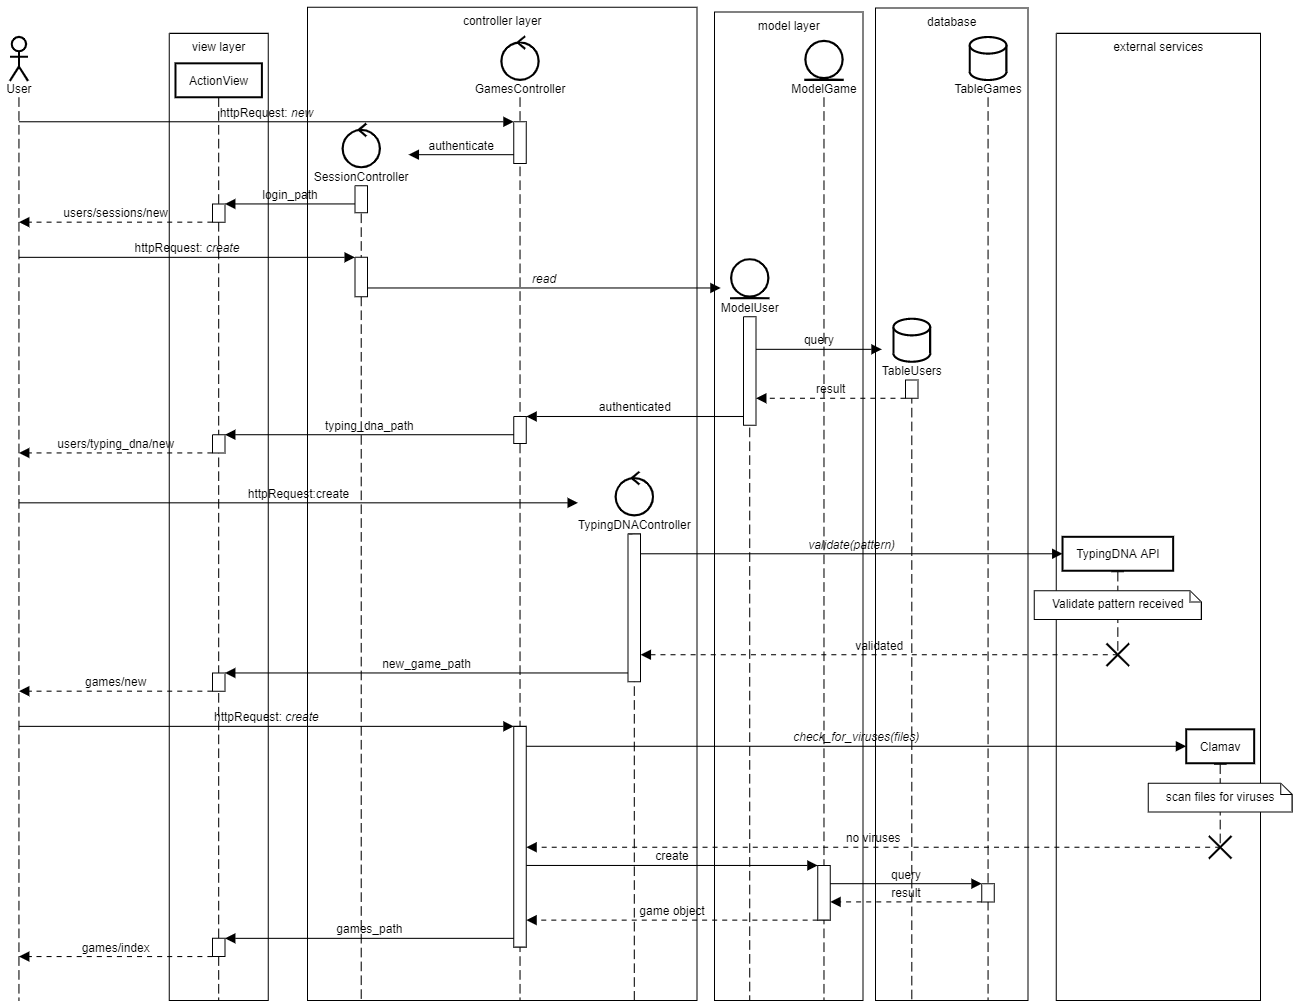
\includegraphics[width=1.2\textwidth]{new_game_sequence_diagram}
    \caption{Diagramma di sequenza: autenticazione e pubblicazione gioco}
\end{figure}